\documentclass{beamer}
\mode<presentation>
{
  \usetheme{ldv}
  \setbeamercovered{transparent}
}

% Uncomment this if you're giving a presentation in german...
\usepackage[ngerman]{babel}

% ...and rename this to "Folie"
\newcommand{\slidenomenclature}{Folie}


\usepackage[utf8]{inputenc}
\usepackage{amsmath,amssymb,amsfonts}
\usepackage{times}
\usepackage{graphicx}
\usepackage{fancyvrb}
\usepackage{array}
\usepackage{colortbl}
\usepackage{tabularx}

% Uncomment me when you need to insert code
\usepackage{color}
\usepackage{listings}
\usepackage{minted}
\usepackage{algpseudocode}
% End Code

\usepackage{datetime}
\usepackage{tikz}

\usetikzlibrary{calc}
\usetikzlibrary{shapes.geometric}
\usetikzlibrary{decorations.pathreplacing}

% Uncomment me when you need video or sound
% \usepackage{multimedia}
% \usepackage{hyperref}
% End video

% Header
\newcommand{\zwischentitel}{Woche 10}
\newcommand{\leitthema}{Tobias Eppacher}
\newcommand{\presdatum}{\formatdate{30}{6}{2025}}
% End Header

% Titlepage
\title{Grundlagen: Algorithmen und Datenstrukturen}
\author{Tobias Eppacher}
\date{\presdatum}
\institute{School of Computation, Information and Technology}
\subtitle{Woche 10}
% End Titlepage


% Slides
\begin{document}


% 1. Slide: Titlepage
\begin{frame}
  \titlepage
\end{frame}

% 2. Slide: TOC
\begin{frame}
  \frametitle{Inhalt}
  \tableofcontents[subsectionstyle=hide]
\end{frame}

\section{Aufgaben}

\begin{frame}
    \frametitle{Aufgabe 10.1 - Hashing mit Chaining}
    \scriptsize
    Veranschaulichen Sie Hashing mit Chaining. Die Größe $m$ der Hash-Tabelle ist in den folgenden Beispielen jeweils die Primzahl $11$. Die folgenden Operationen sollen nacheinander ausgeführt werden:
    \begin{itemize}
      \item insert $3, 11, 9, 7, 14, 56, 4, 12, 15, 8, 1$
      \item delete $56$
      \item insert $25$
    \end{itemize}
    Der Einfachheit halber sollen die Schlüssel der Elemente die Elemente selbst sein.
  
    \medskip
  
    a) Verwenden Sie zunächst die Hashfunktion
    $$g(x) = 5x \mod 11$$
  
    b) Berechnen Sie die Hashwerte unter Verwendung der Hashfunktion
    $$h(x) = \mathbf{a} \cdot \mathbf{x} \mod m$$
  
    nach dem aus der Vorlesung bekannten Verfahren füreinfache universelle Hashfunktionen,
    wobei $\mathbf{a} = (7, 5)$ und $\mathbf{x} = (\lfloor \frac{x}{2^w} \rfloor \mod 2^w, x \mod 2^w)$
    für $w = \lfloor \log_2 m \rfloor = \lfloor 3.45 \dots \rfloor = 3$ gilt
    und der Ausdruck $\mathbf{a} \cdot \mathbf{x}$ ein Skalarprodukt bezeichnet.
  
  \end{frame}
  
  \begin{frame}[t]
    \frametitle{Aufgabe 10.1 - Hashing mit Chaining (a)}
  
    $$g(x) = 5x \mod 11$$
  
    \bigskip
    \bigskip
    \bigskip
    \bigskip
    \bigskip
    \bigskip
    \bigskip
    \bigskip
    \bigskip
    \bigskip
  
    \begin{center}
      \begin{tabular}{c|c|c|c|c|c|c|c|c|c|c|c|c}
        $k(e)$    & 1 & 3 & 4 & 7 & 8 & 9 & 11 & 12 & 14 & 15 & 25 & 56 \\
        \hline
        $g(k(e))$ &   &   &   &   &   &   &    &    &    &    &    &    \\
      \end{tabular}
    \end{center}
  \end{frame}
  
  \begin{frame}
    \frametitle{Aufgabe 10.1 - Hashing mit Chaining (a)}
  
    \begin{center}
      \begin{tabular}{c|c|c|c|c|c|c|c|c|c|c|c|c}
        $k(e)$    & 1 & 3 & 4 & 7 & 8 & 9 & 11 & 12 & 14 & 15 & 25 & 56 \\
        \hline
        $g(k(e))$ & 5 & 4 & 9 & 2 & 7 & 1 & 0  & 5  & 4  & 9  & 4  & 5  \\
      \end{tabular}
    \end{center}
  \end{frame}
  
  \begin{frame}
    \frametitle{Aufgabe 10.1 - Hashing mit Chaining (a)}
  
    1. Operation: insert(3)
  
    \begin{center}
      \begin{tabular}{c|c|c|c|c|c|c|c|c|c|c|c|c}
        $k(e)$    & 1 & 3 & 4 & 7 & 8 & 9 & 11 & 12 & 14 & 15 & 25 & 56 \\
        \hline
        $g(k(e))$ & 5 & 4 & 9 & 2 & 7 & 1 & 0  & 5  & 4  & 9  & 4  & 5  \\
      \end{tabular}
  
      \bigskip
  
      \begin{tabular}{c|c|c|c|c|c|c|c|c|c|c}
        0 & 1 & 2 & 3 & 4 & 5 & 6 & 7 & 8 & 9 & 10 \\
        \hline
          &   &   &   &   &   &   &   &   &   &    \\
          &   &   &   &   &   &   &   &   &   &    \\
          &   &   &   &   &   &   &   &   &   &    \\
      \end{tabular}
    \end{center}
  \end{frame}
  
  \begin{frame}
    \frametitle{Aufgabe 10.1 - Hashing mit Chaining (a)}
    2. Operation: insert(11)
    \begin{center}
      \begin{tabular}{c|c|c|c|c|c|c|c|c|c|c|c|c}
        $k(e)$    & 1 & 3 & 4 & 7 & 8 & 9 & 11 & 12 & 14 & 15 & 25 & 56 \\
        \hline
        $g(k(e))$ & 5 & 4 & 9 & 2 & 7 & 1 & 0  & 5  & 4  & 9  & 4  & 5  \\
      \end{tabular}
  
      \bigskip
  
      \begin{tabular}{c|c|c|c|c|c|c|c|c|c|c}
        0 & 1 & 2 & 3 & 4 & 5 & 6 & 7 & 8 & 9 & 10 \\
        \hline
          &   &   &   & 3 &   &   &   &   &   &    \\
          &   &   &   &   &   &   &   &   &   &    \\
          &   &   &   &   &   &   &   &   &   &    \\
      \end{tabular}
    \end{center}
  \end{frame}
  
  \begin{frame}
    \frametitle{Aufgabe 10.1 - Hashing mit Chaining (a)}
    3. Operation: insert(9)
    \begin{center}
      \begin{tabular}{c|c|c|c|c|c|c|c|c|c|c|c|c}
        $k(e)$    & 1 & 3 & 4 & 7 & 8 & 9 & 11 & 12 & 14 & 15 & 25 & 56 \\
        \hline
        $g(k(e))$ & 5 & 4 & 9 & 2 & 7 & 1 & 0  & 5  & 4  & 9  & 4  & 5  \\
      \end{tabular}
  
      \bigskip
  
      \begin{tabular}{c|c|c|c|c|c|c|c|c|c|c}
        0  & 1 & 2 & 3 & 4 & 5 & 6 & 7 & 8 & 9 & 10 \\
        \hline
        11 &   &   &   & 3 &   &   &   &   &   &    \\
           &   &   &   &   &   &   &   &   &   &    \\
           &   &   &   &   &   &   &   &   &   &    \\
      \end{tabular}
    \end{center}
  \end{frame}
  
  \begin{frame}
    \frametitle{Aufgabe 10.1 - Hashing mit Chaining (a)}
    4. Operation: insert(7)
    \begin{center}
      \begin{tabular}{c|c|c|c|c|c|c|c|c|c|c|c|c}
        $k(e)$    & 1 & 3 & 4 & 7 & 8 & 9 & 11 & 12 & 14 & 15 & 25 & 56 \\
        \hline
        $g(k(e))$ & 5 & 4 & 9 & 2 & 7 & 1 & 0  & 5  & 4  & 9  & 4  & 5  \\
      \end{tabular}
  
      \bigskip
  
      \begin{tabular}{c|c|c|c|c|c|c|c|c|c|c}
        0  & 1 & 2 & 3 & 4 & 5 & 6 & 7 & 8 & 9 & 10 \\
        \hline
        11 & 9 &   &   & 3 &   &   &   &   &   &    \\
           &   &   &   &   &   &   &   &   &   &    \\
           &   &   &   &   &   &   &   &   &   &    \\
      \end{tabular}
    \end{center}
  \end{frame}
  
  \begin{frame}
    \frametitle{Aufgabe 10.1 - Hashing mit Chaining (a)}
    5. Operation: insert(14)
    \begin{center}
      \begin{tabular}{c|c|c|c|c|c|c|c|c|c|c|c|c}
        $k(e)$    & 1 & 3 & 4 & 7 & 8 & 9 & 11 & 12 & 14 & 15 & 25 & 56 \\
        \hline
        $g(k(e))$ & 5 & 4 & 9 & 2 & 7 & 1 & 0  & 5  & 4  & 9  & 4  & 5  \\
      \end{tabular}
  
      \bigskip
  
      \begin{tabular}{c|c|c|c|c|c|c|c|c|c|c}
        0  & 1 & 2 & 3 & 4 & 5 & 6 & 7 & 8 & 9 & 10 \\
        \hline
        11 & 9 & 7 &   & 3 &   &   &   &   &   &    \\
           &   &   &   &   &   &   &   &   &   &    \\
           &   &   &   &   &   &   &   &   &   &    \\
      \end{tabular}
    \end{center}
  \end{frame}
  
  \begin{frame}
    \frametitle{Aufgabe 10.1 - Hashing mit Chaining (a)}
    6. Operation: insert(56)
    \begin{center}
      \begin{tabular}{c|c|c|c|c|c|c|c|c|c|c|c|c}
        $k(e)$    & 1 & 3 & 4 & 7 & 8 & 9 & 11 & 12 & 14 & 15 & 25 & 56 \\
        \hline
        $g(k(e))$ & 5 & 4 & 9 & 2 & 7 & 1 & 0  & 5  & 4  & 9  & 4  & 5  \\
      \end{tabular}
  
      \bigskip
  
      \begin{tabular}{c|c|c|c|c|c|c|c|c|c|c}
        0  & 1 & 2 & 3 & 4  & 5 & 6 & 7 & 8 & 9 & 10 \\
        \hline
        11 & 9 & 7 &   & 3  &   &   &   &   &   &    \\
           &   &   &   & 14 &   &   &   &   &   &    \\
           &   &   &   &    &   &   &   &   &   &    \\
      \end{tabular}
    \end{center}
  \end{frame}
  
  \begin{frame}
    \frametitle{Aufgabe 10.1 - Hashing mit Chaining (a)}
    7. Operation: insert(4)
    \begin{center}
      \begin{tabular}{c|c|c|c|c|c|c|c|c|c|c|c|c}
        $k(e)$    & 1 & 3 & 4 & 7 & 8 & 9 & 11 & 12 & 14 & 15 & 25 & 56 \\
        \hline
        $g(k(e))$ & 5 & 4 & 9 & 2 & 7 & 1 & 0  & 5  & 4  & 9  & 4  & 5  \\
      \end{tabular}
  
      \bigskip
  
      \begin{tabular}{c|c|c|c|c|c|c|c|c|c|c}
        0  & 1 & 2 & 3 & 4  & 5  & 6 & 7 & 8 & 9 & 10 \\
        \hline
        11 & 9 & 7 &   & 3  & 56 &   &   &   &   &    \\
           &   &   &   & 14 &    &   &   &   &   &    \\
           &   &   &   &    &    &   &   &   &   &    \\
      \end{tabular}
    \end{center}
  \end{frame}
  
  \begin{frame}
    \frametitle{Aufgabe 10.1 - Hashing mit Chaining (a)}
    8. Operation: insert(12)
    \begin{center}
      \begin{tabular}{c|c|c|c|c|c|c|c|c|c|c|c|c}
        $k(e)$    & 1 & 3 & 4 & 7 & 8 & 9 & 11 & 12 & 14 & 15 & 25 & 56 \\
        \hline
        $g(k(e))$ & 5 & 4 & 9 & 2 & 7 & 1 & 0  & 5  & 4  & 9  & 4  & 5  \\
      \end{tabular}
  
      \bigskip
  
      \begin{tabular}{c|c|c|c|c|c|c|c|c|c|c}
        0  & 1 & 2 & 3 & 4  & 5  & 6 & 7 & 8 & 9 & 10 \\
        \hline
        11 & 9 & 7 &   & 3  & 56 &   &   &   & 4 &    \\
           &   &   &   & 14 &    &   &   &   &   &    \\
           &   &   &   &    &    &   &   &   &   &    \\
      \end{tabular}
    \end{center}
  \end{frame}
  
  \begin{frame}
    \frametitle{Aufgabe 10.1 - Hashing mit Chaining (a)}
    9. Operation: insert(15)
    \begin{center}
      \begin{tabular}{c|c|c|c|c|c|c|c|c|c|c|c|c}
        $k(e)$    & 1 & 3 & 4 & 7 & 8 & 9 & 11 & 12 & 14 & 15 & 25 & 56 \\
        \hline
        $g(k(e))$ & 5 & 4 & 9 & 2 & 7 & 1 & 0  & 5  & 4  & 9  & 4  & 5  \\
      \end{tabular}
  
      \bigskip
  
      \begin{tabular}{c|c|c|c|c|c|c|c|c|c|c}
        0  & 1 & 2 & 3 & 4  & 5  & 6 & 7 & 8 & 9 & 10 \\
        \hline
        11 & 9 & 7 &   & 3  & 56 &   &   &   & 4 &    \\
           &   &   &   & 14 & 12 &   &   &   &   &    \\
           &   &   &   &    &    &   &   &   &   &    \\
      \end{tabular}
    \end{center}
  \end{frame}
  
  \begin{frame}
    \frametitle{Aufgabe 10.1 - Hashing mit Chaining (a)}
    10. Operation: insert(8)
    \begin{center}
      \begin{tabular}{c|c|c|c|c|c|c|c|c|c|c|c|c}
        $k(e)$    & 1 & 3 & 4 & 7 & 8 & 9 & 11 & 12 & 14 & 15 & 25 & 56 \\
        \hline
        $g(k(e))$ & 5 & 4 & 9 & 2 & 7 & 1 & 0  & 5  & 4  & 9  & 4  & 5  \\
      \end{tabular}
  
      \bigskip
  
      \begin{tabular}{c|c|c|c|c|c|c|c|c|c|c}
        0  & 1 & 2 & 3 & 4  & 5  & 6 & 7 & 8 & 9  & 10 \\
        \hline
        11 & 9 & 7 &   & 3  & 56 &   &   &   & 4  &    \\
           &   &   &   & 14 & 12 &   &   &   & 15 &    \\
           &   &   &   &    &    &   &   &   &    &    \\
      \end{tabular}
    \end{center}
  \end{frame}
  
  \begin{frame}
    \frametitle{Aufgabe 10.1 - Hashing mit Chaining (a)}
    11. Operation: insert(1)
    \begin{center}
      \begin{tabular}{c|c|c|c|c|c|c|c|c|c|c|c|c}
        $k(e)$    & 1 & 3 & 4 & 7 & 8 & 9 & 11 & 12 & 14 & 15 & 25 & 56 \\
        \hline
        $g(k(e))$ & 5 & 4 & 9 & 2 & 7 & 1 & 0  & 5  & 4  & 9  & 4  & 5  \\
      \end{tabular}
  
      \bigskip
  
      \begin{tabular}{c|c|c|c|c|c|c|c|c|c|c}
        0  & 1 & 2 & 3 & 4  & 5  & 6 & 7 & 8 & 9  & 10 \\
        \hline
        11 & 9 & 7 &   & 3  & 56 &   & 8 &   & 4  &    \\
           &   &   &   & 14 & 12 &   &   &   & 15 &    \\
           &   &   &   &    &    &   &   &   &    &    \\
      \end{tabular}
    \end{center}
  \end{frame}
  
  \begin{frame}
    \frametitle{Aufgabe 10.1 - Hashing mit Chaining (a)}
    12. Operation: delete(56)
    \begin{center}
      \begin{tabular}{c|c|c|c|c|c|c|c|c|c|c|c|c}
        $k(e)$    & 1 & 3 & 4 & 7 & 8 & 9 & 11 & 12 & 14 & 15 & 25 & 56 \\
        \hline
        $g(k(e))$ & 5 & 4 & 9 & 2 & 7 & 1 & 0  & 5  & 4  & 9  & 4  & 5  \\
      \end{tabular}
  
      \bigskip
  
      \begin{tabular}{c|c|c|c|c|c|c|c|c|c|c}
        0  & 1 & 2 & 3 & 4  & 5  & 6 & 7 & 8 & 9  & 10 \\
        \hline
        11 & 9 & 7 &   & 3  & 56 &   & 8 &   & 4  &    \\
           &   &   &   & 14 & 12 &   &   &   & 15 &    \\
           &   &   &   &    & 1  &   &   &   &    &    \\
      \end{tabular}
    \end{center}
  \end{frame}
  
  \begin{frame}
    \frametitle{Aufgabe 10.1 - Hashing mit Chaining (a)}
    13. Operation: insert(25)
    \begin{center}
      \begin{tabular}{c|c|c|c|c|c|c|c|c|c|c|c|c}
        $k(e)$    & 1 & 3 & 4 & 7 & 8 & 9 & 11 & 12 & 14 & 15 & 25 & 56 \\
        \hline
        $g(k(e))$ & 5 & 4 & 9 & 2 & 7 & 1 & 0  & 5  & 4  & 9  & 4  & 5  \\
      \end{tabular}
  
      \bigskip
  
      \begin{tabular}{c|c|c|c|c|c|c|c|c|c|c}
        0  & 1 & 2 & 3 & 4  & 5  & 6 & 7 & 8 & 9  & 10 \\
        \hline
        11 & 9 & 7 &   & 3  & 12 &   & 8 &   & 4  &    \\
           &   &   &   & 14 & 1  &   &   &   & 15 &    \\
           &   &   &   &    &    &   &   &   &    &    \\
      \end{tabular}
    \end{center}
  \end{frame}
  
  \begin{frame}
    \frametitle{Aufgabe 10.1 - Hashing mit Chaining (a)}
    13. Operation: insert(25)
    \begin{center}
      \begin{tabular}{c|c|c|c|c|c|c|c|c|c|c|c|c}
        $k(e)$    & 1 & 3 & 4 & 7 & 8 & 9 & 11 & 12 & 14 & 15 & 25 & 56 \\
        \hline
        $g(k(e))$ & 5 & 4 & 9 & 2 & 7 & 1 & 0  & 5  & 4  & 9  & 4  & 5  \\
      \end{tabular}
  
      \bigskip
  
      \begin{tabular}{c|c|c|c|c|c|c|c|c|c|c}
        0  & 1 & 2 & 3 & 4  & 5  & 6 & 7 & 8 & 9  & 10 \\
        \hline
        11 & 9 & 7 &   & 3  & 12 &   & 8 &   & 4  &    \\
           &   &   &   & 14 & 1  &   &   &   & 15 &    \\
           &   &   &   & 25 &    &   &   &   &    &    \\
      \end{tabular}
    \end{center}
  \end{frame}
  
  \begin{frame}
    \frametitle{Aufgabe 10.1 - Hashing mit Chaining (b)}
    b) Berechnen Sie die Hashwerte unter Verwendung der Hashfunktion
    $$h(x) = \mathbf{a} \cdot \mathbf{x} \mod m$$
    nach dem aus der Vorlesung bekannten Verfahren für einfache universelle Hashfunktionen,
    wobei $\mathbf{a} = (7, 5)$ und $\mathbf{x} = (\lfloor \frac{x}{2^w} \rfloor \mod 2^w, x \mod 2^w)$
    für $w = \lfloor \log_2 m \rfloor = \lfloor 3.45 \dots \rfloor = 3$ gilt
    und der Ausdruck $\mathbf{a} \cdot \mathbf{x}$ ein Skalarprodukt bezeichnet.
  
    \bigskip
    \bigskip
  
    \begin{center}
      \begin{tabular}{c|c|c|c|c|c|c|c|c|c|c|c|c}
        $k(e)$    & 1 & 3 & 4 & 7 & 8 & 9 & 11 & 12 & 14 & 15 & 25 & 56 \\
        \hline
        $h(k(e))$ &   &   &   &   &   &   &    &    &    &    &    &    \\
      \end{tabular}
    \end{center}
  \end{frame}
  
  \begin{frame}[t]
    \frametitle{Aufgabe 10.1 - Hashing mit Chaining (b)}
    $$h(x) = \mathbf{a} \cdot \mathbf{x} \mod m$$
    $$\mathbf{a} = (7, 5) \qquad \mathbf{x} = \left(\lfloor \frac{x}{2^w} \rfloor \mod 2^w, x \mod 2^w\right) $$
  
    \bigskip
    \bigskip
    \bigskip
    \bigskip
    \bigskip
    \bigskip
    \bigskip
    \bigskip
  
    \begin{center}
      \begin{tabular}{c|c|c|c|c|c|c|c|c|c|c|c|c}
        $k(e)$    & 1 & 3 & 4 & 7 & 8 & 9 & 11 & 12 & 14 & 15 & 25 & 56 \\
        \hline
        $h(k(e))$ &   &   &   &   &   &   &    &    &    &    &    &    \\
      \end{tabular}
    \end{center}
  \end{frame}
  
  \begin{frame}
    \frametitle{Aufgabe 10.1 - Hashing mit Chaining (b)}
    \begin{center}
      \begin{tabular}{c|c|c|c|c|c|c|c|c|c|c|c|c}
        $k(e)$    & 1 & 3 & 4 & 7 & 8 & 9 & 11 & 12 & 14 & 15 & 25 & 56 \\
        \hline
        $h(k(e))$ & 5 & 4 & 9 & 2 & 7 & 1 & 0  & 5  & 4  & 9  & 4  & 5  \\
      \end{tabular}
    \end{center}
  \end{frame}

\begin{frame}
  \frametitle{Aufgabe 10.2 - B-Baum Analyse (Viel Text)}
  \small
  Der Aufwand nach dem Einfügen oder Entfernen einen perfekt balancierten Binärbaum
  wiederherzustellen ist $\mathcal{O}(n)$ im Worstcase. Daher versuchen AVL-Bäume keinen perfekt
  balancierten Binärbaum zu erreichen sondern stellen lediglich einen möglichst gut balancierten
  Binärbaum sicher.

  \medskip
  Die Tiefe eines AVL-Baums ist dabei im Worstcase $1.44 \ast \log_2(n)$ und bei
  einem Rot-Schwarz-Baum $2 \ast \log_2(n)$. Diese Tiefe ist bei Binärbäumen auch die maximale
  Anzahl an notwendigen Vergleichen z.B. beim Suchen eines Werts.

  \medskip
  Wir wollen nun so eine Analyse für einen B-Baum machen. B-Bäume sind eng verwandt mit
  den AB-Bäumen. Ein $k$-Baum ist dasselbe wie ein $k$,$2k$-Baum, bei einem B-Baum ist also
  die Obergrenze fur die Anzahl der Kinder eines Knoten genau das Doppelte.

\end{frame}

\begin{frame}[t]
  \frametitle{Aufgabe 10.2 - B-Baum Analyse (a)}
  Wie ist ein Baum aufgebaut, der die größt mögliche Tiefe mit der kleinst möglichen Anzahl
  an Elementen erreicht?

  \smallskip
  Schätzen Sie die notwendigen Vergleiche im Worstcase für eine Suche nach einem Wert in
  diesem Baum ab.

  \smallskip
  \textbf{Hinweis:} Es müssen dabei nicht alle Werte aus einem Knoten betrachtet werden.
\end{frame}

\begin{frame}
  \frametitle{Aufgabe 10.2 - B-Baum Analyse (a)}
\end{frame}

\begin{frame}[t]
  \frametitle{Aufgabe 10.2 - B-Baum Analyse (b)}
  Wie sieht der Baum aus, sodass möglichst viele Vergleiche im Worstcase im Verhältnis
  zu der Anzahl von Elementen im Baum notwendig sind bei der Suche nach einem
  Wert?

  \smallskip
  Wie viele Vergleiche sind nun im Worstcase schätzungsweise nötig?
\end{frame}

\begin{frame}
  \frametitle{Aufgabe 10.2 - B-Baum Analyse (b)}
\end{frame}

\begin{frame}[t]
  \frametitle{Aufgabe 10.2 - B-Baum Analyse (c)}

  Wie verhält sich die notwendige Anzahl an Vergleichen bei wachsenden $k$?

  \smallskip
  Erkläre warum sich die Anzahl der Vergleiche so verhält.
\end{frame}

\begin{frame}
  \frametitle{Aufgabe 10.2 - B-Baum Analyse (c)}
\end{frame}

\begin{frame}
  \frametitle{Aufgabe 10.3 - Klausurvorbereitung: Transfer}

  \begin{enumerate}
    \renewcommand{\theenumi}{\alph{enumi}}
    \item Wie viele verschiedene Baumstrukturen sind mit $11$ Elementen bei einem $3$,$5$-Baum
          möglich?
    \item Wie viele verschiedene Baumstrukturen sind bei einem $3$-Baum ($3$,$6$-Baum) mit $3$
          Ebenen möglich?
  \end{enumerate}
\end{frame}

\begin{frame}[t]
  \frametitle{Aufgabe 10.3 - Klausurvorbereitung: Transfer (a)}

  Wie viele verschiedene Baumstrukturen sind mit $11$ Elementen bei einem $3$,$5$-Baum möglich?
\end{frame}

\begin{frame}[t]
  \frametitle{Aufgabe 10.3 - Klausurvorbereitung: Transfer (a)}

  Wie viele verschiedene Baumstrukturen sind mit $11$ Elementen bei einem $3$,$5$-Baum möglich?
\end{frame}

\begin{frame}[t]
  \frametitle{Aufgabe 10.3 - Klausurvorbereitung: Transfer (b)}

  Wie viele verschiedene Baumstrukturen sind bei einem $3$-Baum ($3$,$6$-Baum) mit $3$ Ebenen möglich?
\end{frame}

\begin{frame}[t]
  \frametitle{Aufgabe 10.3 - Klausurvorbereitung: Transfer (b)}

  Wie viele verschiedene Baumstrukturen sind bei einem $3$-Baum ($3$,$6$-Baum) mit $3$ Ebenen möglich?
\end{frame}

\begin{frame}
  \frametitle{Aufgabe 10.4 - Klausurvorbereitung: Fehlersuche}

  Schauen Sie sich folgende drei Methoden an, die einen Algorithmus aus der Vorlesung implementiert haben. Beschreiben Sie welcher Algorithmus implementiert wurde und was dessen
  Laufzeit sein sollte. Geben Sie zudem den oder die Fehler in den gegebenen Methoden an
  und beschreiben Sie welche Auswirkungen die Fehler auf die Laufzeit und/oder das Ergebnis
  der Methoden haben. Beschreiben sie zudem, wie der Code verändert werden muss, um den
  Fehler zu beheben. Sind diese Methoden genau so performant wie die Implementierung aus
  der Vorlesung?
\end{frame}

\begin{frame}
  \frametitle{Aufgabe 10.4 - Klausurvorbereitung: Fehlersuche}
  \small
  a) Methode 1:

  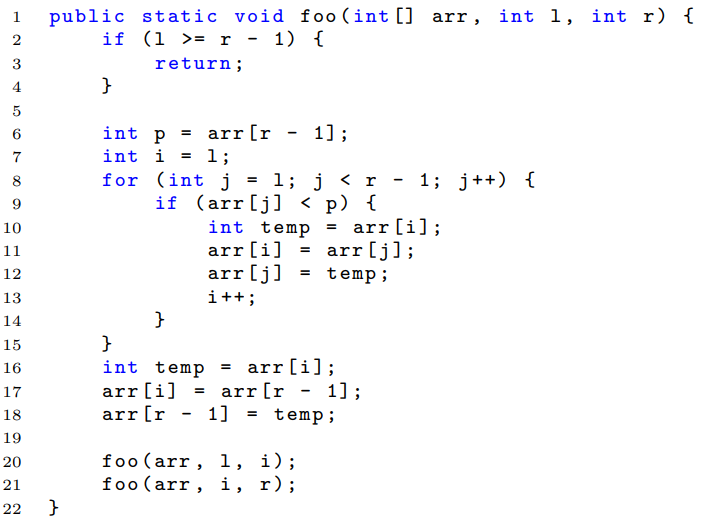
\includegraphics[scale=0.45]{images/10_4_a.png}
\end{frame}

\begin{frame}
  \frametitle{Aufgabe 10.4 - Klausurvorbereitung: Fehlersuche}
  \small
  b) Methode 2:


  \bigskip
  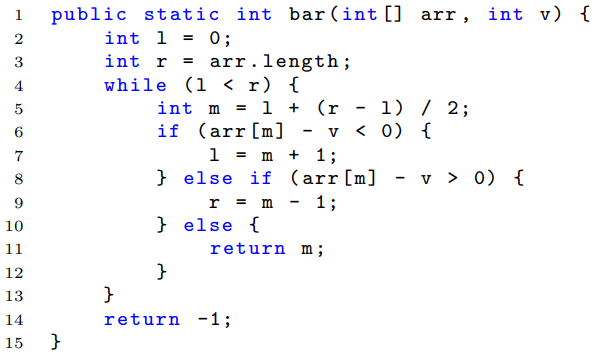
\includegraphics[scale=0.45]{images/10_4_b.png}
\end{frame}

\begin{frame}
  \frametitle{Aufgabe 10.4 - Klausurvorbereitung: Fehlersuche}
  \small
  c) Methode 3:

  \smallskip
  \textit{stream} erzeugt dabei einen Stream aus dem übergebenen Arrray, \textit{of} gibt
  einen Stream zurück, der nur den angegebenen Wert enthält, und \textit{concat} konkateniert
  zwei Streams zu einem längeren.

  \bigskip
  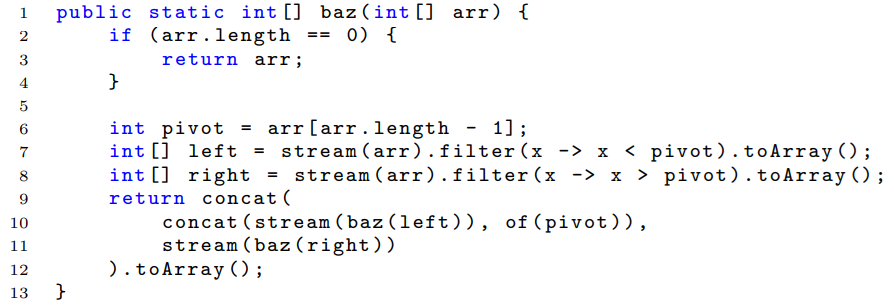
\includegraphics[scale=0.45]{images/10_4_c.png}
\end{frame}

\section{E-Aufgaben}
\begin{frame}
  \frametitle{E-Aufgaben}
  \begin{itemize}
    \item Aufgabe 10.5 - Chaining 2 \\
          \begin{itemize}
            \item Hashing mit Chaining Wiederholung
          \end{itemize}
    \item Aufgabe 10.6 - Klausurvorbereitung: Transfer 2 \\
          \begin{itemize}
            \item Theoriefragen zu Bäumen
          \end{itemize}
  \end{itemize}
\end{frame}

\section{Hausaufgaben}
\begin{frame}
  \frametitle{Hausaufgaben}
  \begin{itemize}
    \item Hausaufgabe 8 - AVL Baum \\
          (Deadline: 02.07.2025)
    \item Hausaufgabe 9 - AB-Baum \\
          (Deadline: 09.07.2025)
    \item Hausaufgabe 10 - Simple Hashing with Chaining \\
          (Deadline: 16.07.2025)
  \end{itemize}
\end{frame}

\begin{frame}
  \textbf{Fragen?}
  \begin{itemize}
    \item Nach Übung gerne bei mir melden
    \item Tutoriumschannel oder DM an mich auf Zulip
    \item Vorlesungschannels von GAD auf Zulip (insbesondere bei Hausaufgaben)
  \end{itemize}

  \medskip
  \textbf{Feedback oder Verbesserungsvorschläge?} \\
  Gerne nach dem Tutorium mit mir quatschen oder DM auf Zulip

  \medskip
  \textbf{Bis nächste Woche!}
\end{frame}

% End Slides

\end{document}
